\section{Diagramma delle classi}
L'applicazione SWEDesigner permette di generare un codice Java funzionante a partire da Diagrammi delle classi e diagrammi delle attività.\\
In questa sezione verranno presentati le funzionalità principali offerte dall'applicazione per quanto riguarda la realizzazione di diagrammi delle classi.

\subsection{Inserimento elementi classi}
Per inserire un elemento per la realizzazione del diagramma delle classi è sufficiente selezionare dalla barra laterale di sinistra, uno degli elementi desiderati, e posizionarlo nell'area di disegno effettuando un clic sulla posizione voluta.
\begin{figure}[h!]
	\centering
		\includegraphics[scale=1]{../img/addClass.png}
	\caption{Inserimento classe}
\end{figure}
\newpage

\subsection{Modificare una classe}
Per modificare una classe, una volta cliccato sulla classe desiderata, a destra compare un menu di modifica.
\begin{figure}[h!]
	\centering
		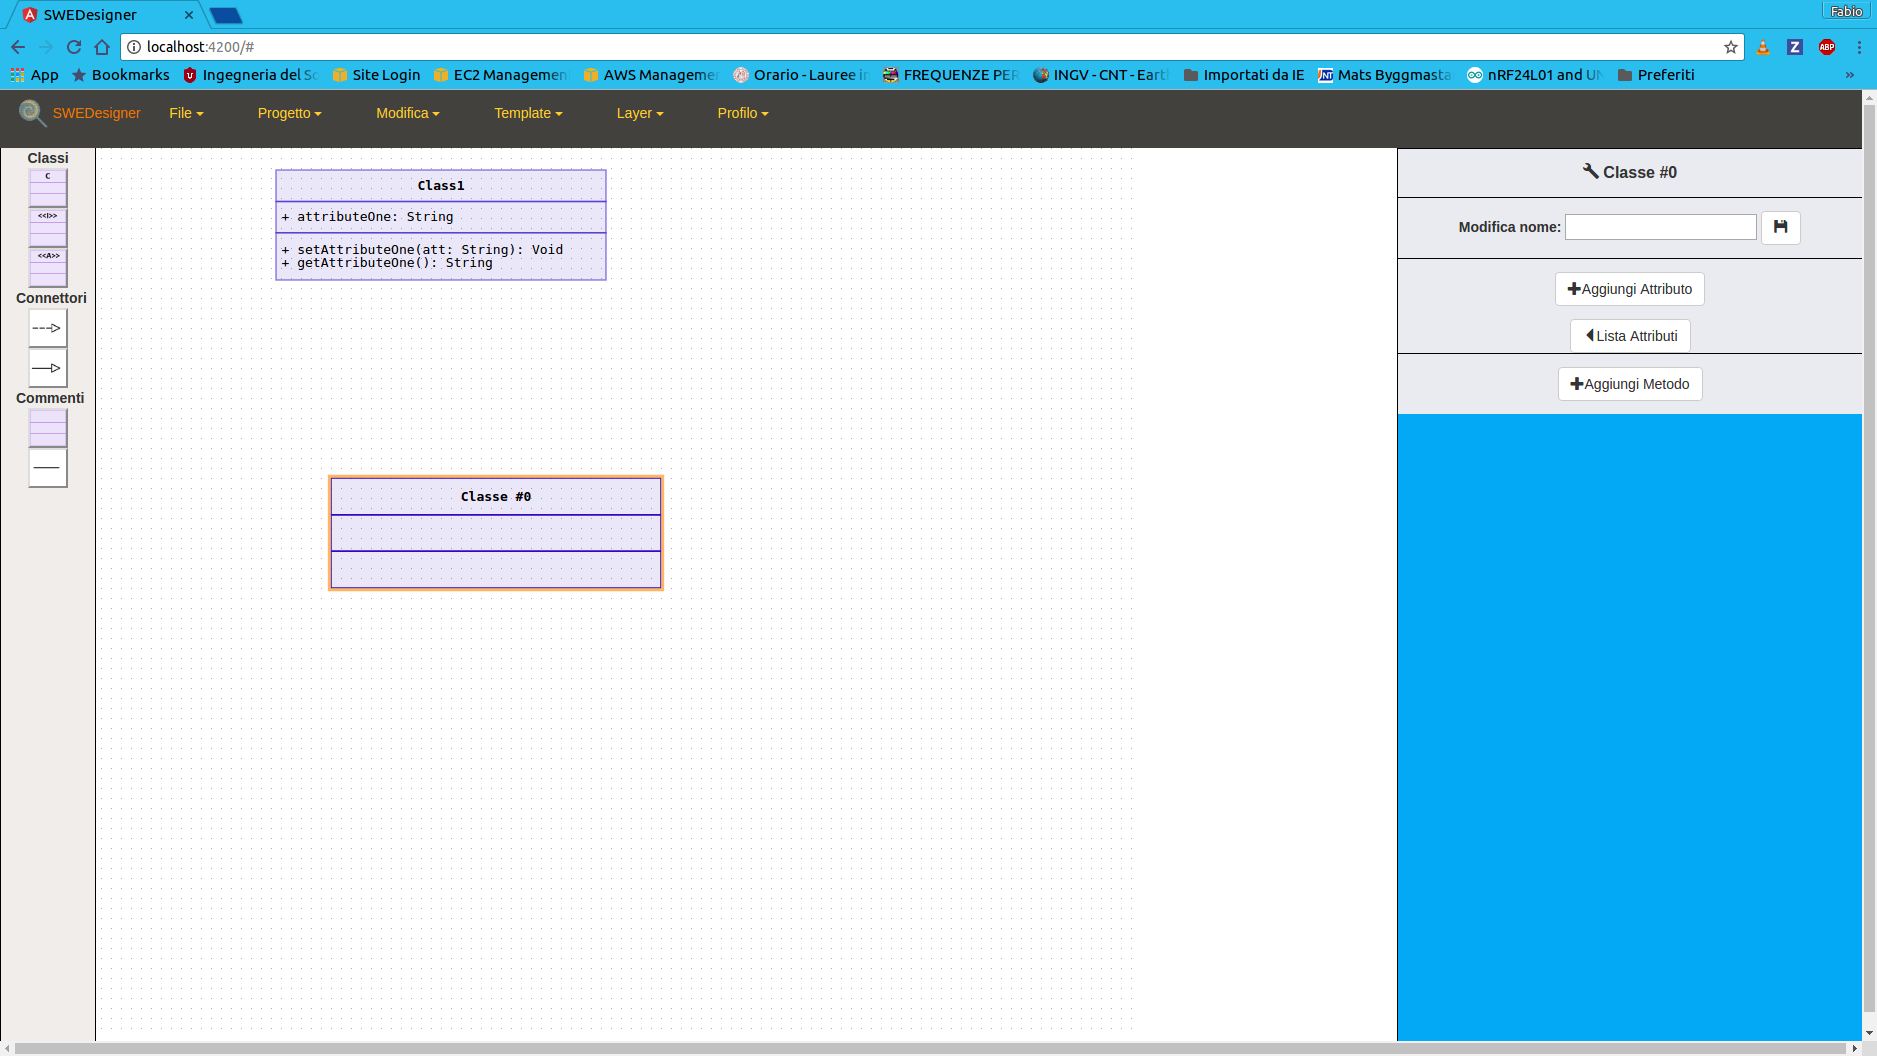
\includegraphics[scale=1]{../img/editClass.png}
	\caption{Zoom}
\end{figure}
\newpage

\subsubsection{Gestione Attributi}
É possibile visualizzare una lista di tutti gli attributi attualmente inseriti, potendoli modificare, o aggiungerne di nuovo, compilando i form con i relativi dati.
\begin{figure}[h!]
	\centering
		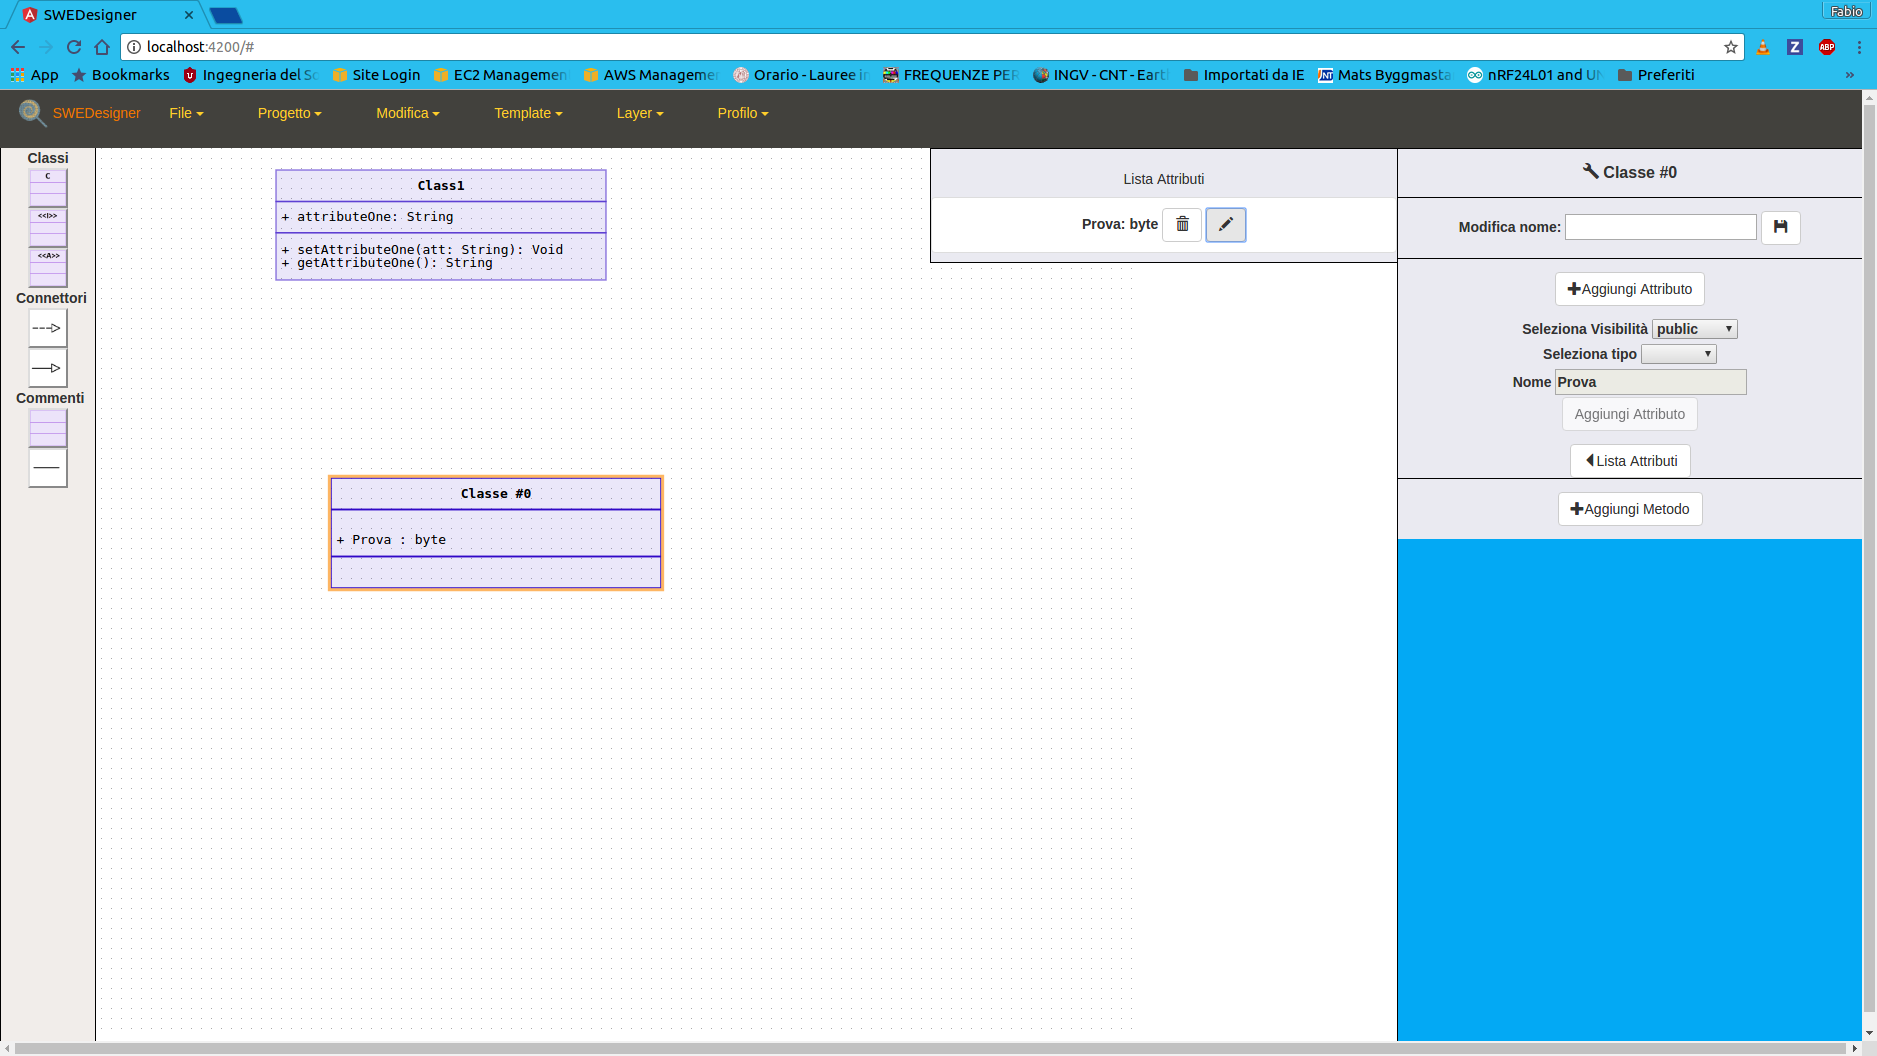
\includegraphics[scale=1]{../img/modAttrib.png}
	\caption{Gestione Attributi}
\end{figure}
\newpage

\subsubsection{Gestione Metodi}
É possibile visualizzare una lista di tutti i metodi attualmente inseriti, potendoli modificare, o aggiungerne di nuovo, compilando i form con i relativi dati. Selezionando il l'icona di modifica, è possibile entrare nella modalità di disegno dei diagrammi delle attività.
\begin{figure}[h!]
	\centering
		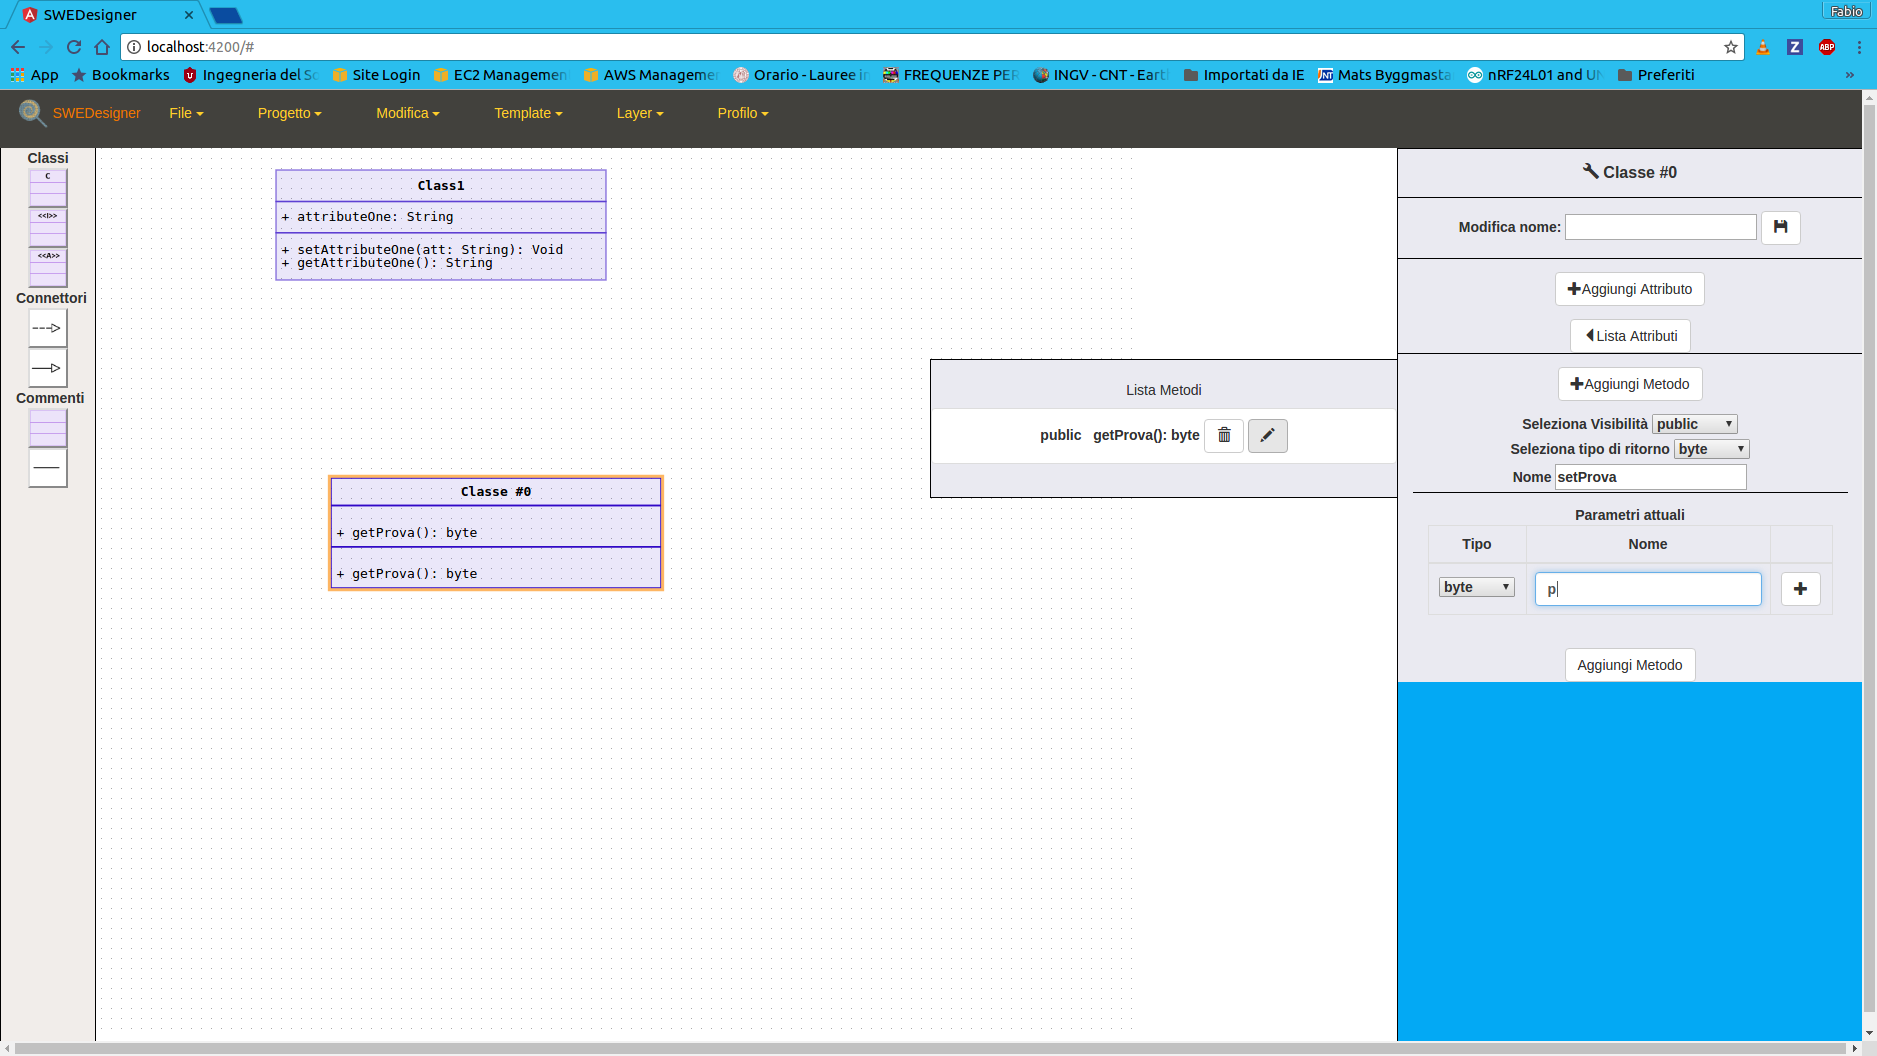
\includegraphics[scale=1]{../img/editMetod.png}
	\caption{Gestione Metodi}
\end{figure}